\documentclass[a4paper,12pt]{article}
\usepackage{blindtext}
\usepackage[utf8]{inputenc}
\usepackage{graphicx}
\usepackage{array}
\newcolumntype{L}{>{\raggedright\arraybackslash}m{8cm}}

\begin{document}
\section{Functional Requirements}

\subsection{System Modules}
\subsubsection{Locations}
This module will be responsible for everything location related. It will store data about locations such as GPS coordinates, it's name, whether its a point of interest or not. This module will also be responsible for storing user specified locations and provide services such as determining their current location and finding locations. This module will also store the UP calendar and allow the updating of event and activity locations. Some of the functionality provided by this is as follows:
\begin{itemize}
\item \textbf{GetLocation -} This function retrieves the GPS coordinates of a certain location. This is a critical function.
\item \textbf{SearchLocation -} This function searches for a location and if found returns its GPS coordinates. This function is critical
\item \textbf{SaveLocation -} This function saves a location. This function is important.
\item \textbf{GetActivity -} This function gets an activity available on campus and provides the user with its time and location. This function is nice-to-have.
\end{itemize}

\subsubsection{Routes}
This module will be responsible for determining routes and providing navigation between locations. The module will determine all routes from locations as well as determine the optimal route. This module will also display the user with a map as they navigate their way around campus. The module will also store most requested routes and the routes between frequently visited locations. Routes will be identified using their starting and end locations. Some of the functionality provided by this module will be:
\begin{itemize}
\item \textbf{GetDirections -} This function determines the routes from one place to another. This function is critical.
\item \textbf{StoreRoute - } This function will store a route when it is frequented often. This function is important.
\item \textbf{GetStoredRoute - } This function will fetch a stored route. This function is important.
\end{itemize}

\subsubsection{Traffic}
This module will be responsible for traffic. This is the surveillance and determination of traffic conditions whether by using cameras or crowd-sourcing. This module will also store which locations are usually heavily populated and at what times. This module will also push traffic notifications to users who request it. In addition to that, users currently using the map to navigate will also be provided with a heat map that displays traffic conditions to them. Some of the functionality provided by this module is described:
\begin{itemize}
\item \textbf{DetermineTraffic -} This function determines the traffic on a specified route. This function is important.
\item \textbf{ShowTraffic -} This function displays the traffic conditions to the user. This function is nice-to-have.
\end{itemize}

\subsubsection{Users}
This module will be responsible for user information. This will store user information such as log in credentials, if they participate in activities, user schedules, user preferences and other information. This module will be responsible for providing the users preferences while using the application to get routes and navigation. This module will also be used by activities to update user information and enable interaction among other users. Some of the functionality provided by the module are: 
\begin{itemize}
\item \textbf{CheckUserCredentials -} This function checks inputted user credentials against stored credentials to authenticate users. This function is important.
\item \textbf{GetUserLocation -} This function gives the users current location in GPS coordinates. This function is critical.
\item \textbf{GetPreferences -} This function gets the users preferences. This function is important.
\item \textbf{SetPreferences -} This function sets and stores the users preferences. This function is important.
\end{itemize}

\subsubsection{Activities}
This module will be centered around extra features of the application not centered around navigation. This will include activities such as steps taken, calories burnt, distance covered and the like. This module could also include a explore campus function which takes the user around campus to discover new things by selecting random locations. This module will allow interaction between users.
 
\subsubsection{Notifications}
This module will be responsible for notifying users. This module will require scheduling functionality in order to push notifications at appropriate times. Notifications will be requested by other modules and will set up the information required for the notification. Some of the functionality to be provided by this module is:
\begin{itemize}
\item \textbf{NotifyUser -} This function sends push notifications to the user. This function is nice-to-have.
\end{itemize}

\subsection{Use Cases}
In this section, we describe each key feature that the system shall provide and the functional requirements for that feature. The functional requirements are the functions, inputs and outputs required for a feature or use case to be achieved. 
\subsubsection{FindVenue Use Case}
\textbf{Description: } This use case helps the user to find a venue on campus\\
\textbf{Priority Level: } Critical\\
\textbf{Inputs:} Name of venue\\
\textbf{Outputs:} Location of inputted venue\\
\textbf{Use case diagram: }\\
%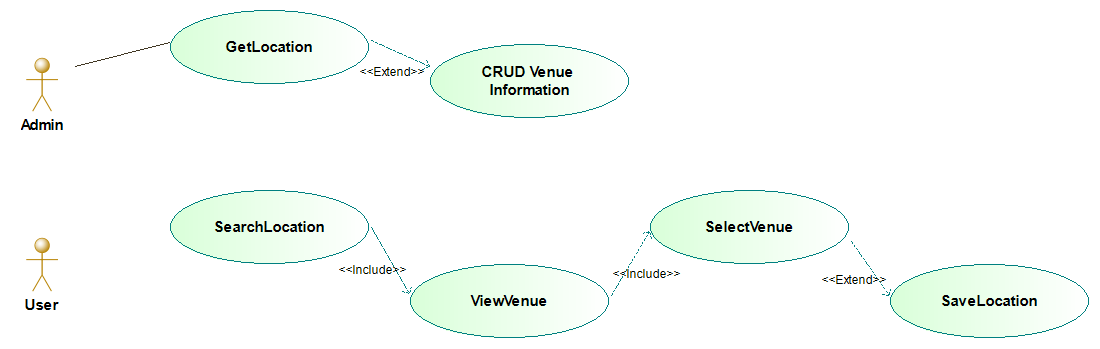
\includegraphics[width=\textwidth]{images/find_venue.jpg}

\subsubsection{FindService Use Case}
\textbf{Description: } This use case helps the user to find a service that is available on campus\\
\textbf{Priority Level:} Important\\
\textbf{Inputs:} A service\\
\textbf{Outputs:} Location of inputted service\\
\textbf{Use case diagram: }\\
%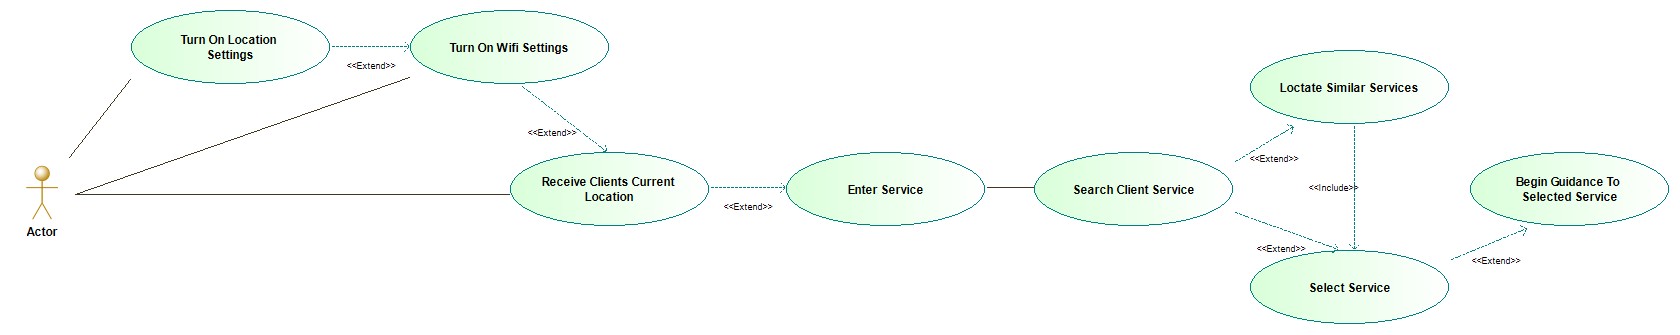
\includegraphics[width=\textwidth]{images/find_service.jpg}

\subsubsection{FindActivity Use Case}
\textbf{Description: } This use case helps the user to find activities at UP to participate in\\
\textbf{Priority Level: } Nice-to-Have\\
\textbf{Inputs:} Type of activity to be searched for\\
\textbf{Outputs:} Activities available with activity time and activity location\\
\textbf{Use case diagram: }\\
%\includegraphics[width=\textwidth]{images/find_activity.jpg}

\subsubsection{ProvideRoute Use Case}
\textbf{Description: } This use case provides a route from a location on campus (which could be the user's current location or specified) to another location on campus (which could be specified or returned by FindVenue, FindService or FindActivity).\\
\textbf{Priority Level: } Critical\\
\textbf{Inputs:} From Where and To Where\\
\textbf{Outputs:} Route from a place to another place\\
\textbf{Use case diagram: }\\
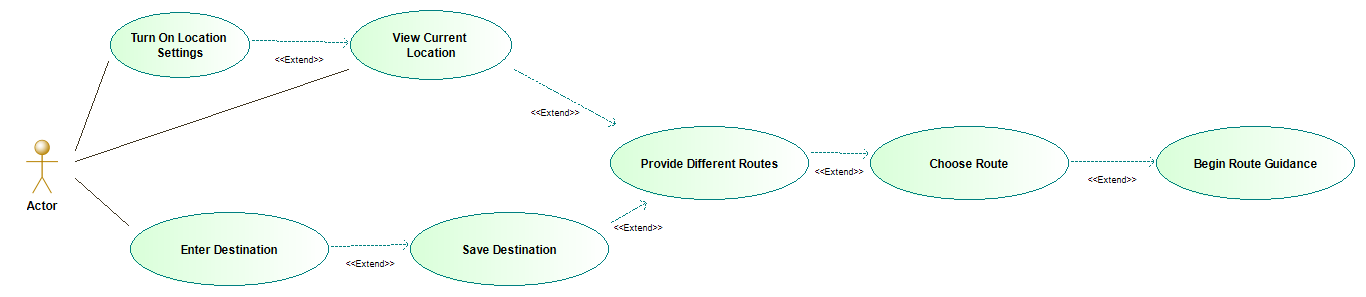
\includegraphics[width=\textwidth]{images/provide_route.png}

\subsubsection{ProvideOptimalRoute Use Case}
\textbf{Description: } This use case provides the best route from a location on campus to another location on campus. "Best" route being determined by user specified factors such as if traffic should be avoided or if the student center should be passed on the way\\
\textbf{Priority Level: } Important\\
\textbf{Inputs:} From Where, To Where and User Preferences\\
\textbf{Outputs:} Optimal route from a place to another place\\
\textbf{Use case diagram: }\\
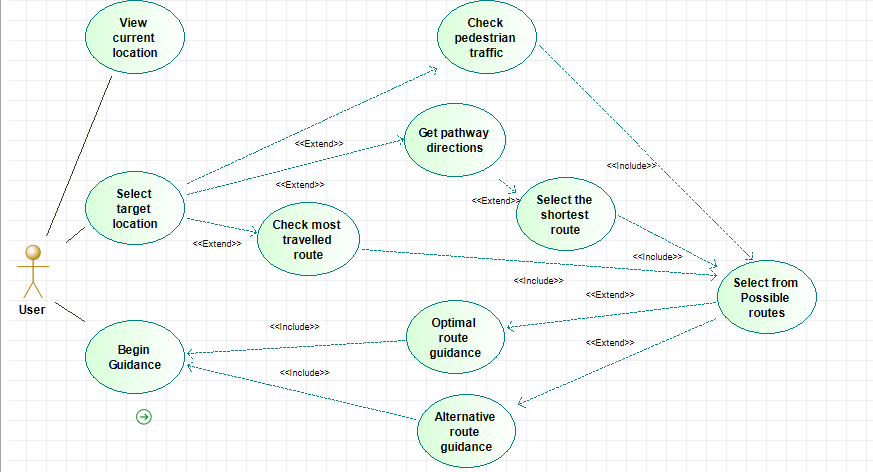
\includegraphics[width=\textwidth]{images/op_route.png}

\subsection{Actor-System Interaction}

\begin{table}[!htbp]
\footnotesize
\label{tab:table 2.2}
\bgroup
\def\arraystretch{1.3}
\begin{tabular}{|L|L|}
\hline
\textbf{\textit{ACTOR - USER}} & \textbf{\textit{SYSTEM - UP NAV}}
\\
\hline
\textbf{1.} User opens application \linebreak \linebreak
\textbf{Precondition:} User does not know how to get somewhere. & \textbf{2.} Application opens on mobile device and lists all options for navigation. \linebreak \linebreak
\textbf{Precondition:} No user input has been given so a default screen is displayed.
\\
\hline
\textbf{3.} User successfully identifies the navigation option from start menu \linebreak \linebreak
& \textbf{4.} System prompts user for destination to navigate to. \linebreak \linebreak
\textbf{Postcondition:} After determining the user's location it can start searching for possible path for the destination.
\\
\hline
\textbf{5.} User adds a criteria (e.g. avoid traffic) to refine the route \linebreak \linebreak
\textbf{Postcondition:} Adding extra information results in a better path.
& \textbf{6.} System chooses a single route and prepares step-by-step instructions to deliver to the user telling them how to arrive at their destination. \linebreak \linebreak 
\textbf{Postcondition:} The GUI will display the route to the user and real-time navigation will begin as the user starts following the given directions.
\\
\hline
\textbf{7.} User follows push notifications and prompts along the chosen route \linebreak
& \textbf{8.} System tracks the user's movement, checking whether their movements correspond to the path given. \linebreak
\\
\hline
\textbf{9.} User strays from given route \linebreak \linebreak
\textbf{Postcondition:} User is no longer following the route and might not arrive at destination.
& \textbf{10.} Constantly tracking the user as he/she moves the application can see that the user is no longer on route and will prompt the user to go back onto the original path or suggest alternatives to follow. \linebreak \linebreak
\\
\hline
\textbf{11.} User gets back onto the right route and arrives at destination \linebreak \linebreak
\textbf{Precondition:} The user was following the wrong path \linebreak 
\textbf{Postcondition:} The user now follows the path that will lead to their destination.
& \textbf{12.} System alerts user that they have arrived at their destination through some visual feedback and exits the navigational mode. \linebreak
\\
\hline	
\end{tabular}
\egroup	
\end{table}

\subsection{Traceability Matrix}
The traceability matrix visually depicts the functional requirements and their priority in relation to the use cases and their priority. \\
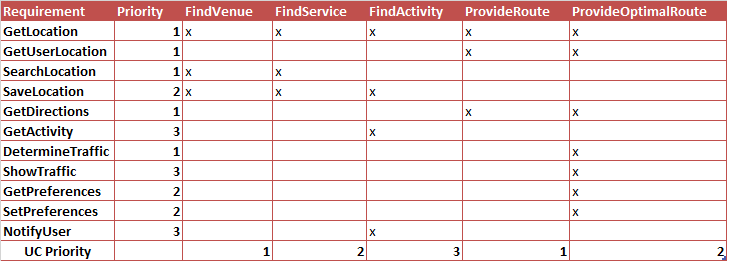
\includegraphics[width=\textwidth]{images/trmatrix.png}
\end{document}